\documentclass[11pt]{article}
\usepackage[a4paper,margin=2.3cm]{geometry}
\usepackage[T1]{fontenc}
\usepackage{lmodern}
\usepackage{microtype}
\usepackage{amsmath}
\usepackage{booktabs}
\usepackage{graphicx}
\usepackage{tabularx}
\usepackage{xcolor}
\usepackage[hidelinks]{hyperref}
\usepackage{caption}
\usepackage[round]{natbib}
\captionsetup{font=small,labelfont=bf}
\setlength{\parskip}{0.35em}
\graphicspath{{../results/}}
% Generated by report/build_numbers.py -- do not edit.
\newcommand{\EnfN}{13}
\newcommand{\EnfMatch}{13}
\newcommand{\EnfRows}{S1 & farmer $\to$ approved vendor & \texttt{tesSUCCESS} & - \\
S2 & farmer $\to$ farmer (direct payment) & \texttt{tecNO\_PERMISSION} & L1: DepositAuth on receiver \\
S3 & farmer $\to$ unauthorized account & \texttt{tecPATH\_DRY} & L1: RequireAuth on issuer \\
S4a & ripple CRD through farmer B, trust-line flags as created & \texttt{tesSUCCESS; B CRD +10} & nobody: B's issuer line is created without NoRipple \\
S4b & same, after NoRipple is set on B's issuer line & \texttt{tecPATH\_DRY; B CRD +0} & L1: NoRipple on both of B's lines \\
S4c & same, after B clears that NoRipple again & \texttt{tesSUCCESS; B CRD +10} & nobody on L1: B controls its own NoRipple flag \\
S5 & farmer clears own DepositAuth, then farmer $\to$ farmer & \texttt{tesSUCCESS} & nobody on L1: depends on who holds the farmer's key \\
S6a & farmer sells credit for XRP on the open DEX, farmer buys & \texttt{tesSUCCESS; B CRD +10} & nobody on L1: offers bypass DepositAuth \\
S6b & farmer places an offer in the vendor-only permissioned DEX & \texttt{tecNO\_PERMISSION} & L1: Permissioned DEX membership \\
S6c & control: vendor places an offer in the same domain & \texttt{tesSUCCESS} & - \\
S7 & farmer and vendor settle off-ledger & \texttt{not observable} & field: audits, vendor incentives \\
S8a & issuer freezes farmer A's line; A $\to$ vendor & \texttt{tecPATH\_DRY} & L1: issuer Freeze \\
S8b & issuer claws back 5 CRD from farmer A & \texttt{tesSUCCESS; A CRD -5} & L1: issuer Clawback \\}
\newcommand{\GapRows}{Risk-aware greedy & 99.6 & 99.0--100.0 \\
Budget-only greedy & 84.0 & 82.5--84.9 \\
Equal amounts & 73.1 & 70.4--74.7 \\
Proportional to farm size & 65.4 & 64.4--66.8 \\
Random, best of 200 & 57.3 & 55.5--58.9 \\
Random, mean of 200 & 52.4 & 50.9--53.1 \\}
\newcommand{\NInst}{20}
\newcommand{\GreedyRiskMed}{99.6}
\newcommand{\GreedyRiskMin}{99.0}
\newcommand{\GreedyMed}{84.0}
\newcommand{\GreedyTightest}{50}
\newcommand{\MilpSecs}{0.5}
\newcommand{\SimReps}{1,000}
\newcommand{\SimRows}{RCT-like (1.0) & custodial & 0.58 & 0.68 & 0.79 & 1.26 & +16.1\% & 0.63 \\
RCT-like (1.0) & self-custody & 0.37 & 0.42 & 0.47 & 0.83 & +12.0\% & 0.56 \\
Trial plots (3.58) & custodial & 3.43 & 4.08 & 4.62 & 5.20 & +13.2\% & 0.88 \\
Trial plots (3.58) & self-custody & 1.67 & 1.96 & 2.24 & 3.25 & +14.7\% & 0.65 \\
Naive agronomic (8.8) & custodial & 9.78 & 12.30 & 12.47 & 13.47 & +1.4\% & 1.04 \\
Naive agronomic (8.8) & self-custody & 4.77 & 5.46 & 6.32 & 8.24 & +15.8\% & 0.71 \\}
\newcommand{\TargetLo}{14}
\newcommand{\TargetHi}{26}
\newcommand{\LedgerLo}{12}
\newcommand{\LedgerHi}{16}
\newcommand{\LedgerMin}{1.4}
\newcommand{\CustodyLo}{40}
\newcommand{\CustodyHi}{51}
\newcommand{\FundRctLo}{54}
\newcommand{\FundRctHi}{69}
\newcommand{\RctLedgerPct}{16}
\newcommand{\RctTypePct}{84}
\newcommand{\AucRows}{None (pooled rate) & 0.500 & 0.500 \\
Land & 0.538 & 0.522 \\
+ loan and default history & 0.693 & 0.630 \\
+ on-ledger diversion & 0.694 & 0.634 \\
+ all diversion (not observable) & 0.696 & 0.639 \\
Known repayment type (benchmark) & 0.693 & 0.672 \\}
\newcommand{\RiskReps}{100}
\newcommand{\ObsZero}{+14.1\%}
\newcommand{\ObsFull}{+15.1\%}
\newcommand{\GbmAuc}{0.657}
\newcommand{\LogAuc}{0.694}
\newcommand{\CalLoPred}{0.15}
\newcommand{\CalLoObs}{0.20}
\newcommand{\CalHiPred}{0.59}
\newcommand{\CalHiObs}{0.55}
\newcommand{\SensReps}{500}
\newcommand{\SensLedgerLo}{0.04}
\newcommand{\SensLedgerHi}{31.8}
\newcommand{\SensCustLo}{23}
\newcommand{\SensCustHi}{69}
\newcommand{\SensFundLo}{0.62}
\newcommand{\SensFundHi}{1.23}
\newcommand{\SensTargetLo}{10.8}
\newcommand{\SensTargetHi}{37.4}
\newcommand{\SensDefLow}{0.04}
\newcommand{\SensDefHigh}{31.8}
\newcommand{\SensCapLoose}{0.9}
\newcommand{\SensCapTight}{30.1}
\newcommand{\PowerRows}{20 & 6.8 & 9.0 & 11.8 \\
40 & 4.8 & 6.4 & 8.3 \\
80 & 3.4 & 4.5 & 5.9 \\}
\newcommand{\PowerBaseDefault}{0.18}
\newcommand{\EffLedgerPP}{1.4}
\newcommand{\EffCustodyPP}{11.2}


\title{\textbf{Restricted-Spend Input Credit on the XRP Ledger}\\[0.3em]
\large Enforcement Tests and a Simulation of a Revolving Credit Fund}
\author{Veysel G\"uzels\"oz\\
\small Wroc\l{}aw University of Science and Technology\\
\small \href{mailto:veyselguzelsoz1@gmail.com}{veyselguzelsoz1@gmail.com}}
\date{Working note, October 2026}

\begin{document}
\maketitle

\begin{abstract}
\noindent
This note looks at credit that is given to smallholder farmers as a token that can only be
spent with approved input vendors. I study two questions: what the blockchain itself can
enforce, and how useful the repayment history on the ledger is for a lender. First, I ran
\EnfN{} scenarios with real transactions on the XRP Ledger testnet to see which spending
restrictions the protocol enforces and which ones depend on who holds the farmer's key, on
the issuer, or on checks in the field. Second, I formulated credit allocation under a budget
and a cap on expected loss, and compared an exact solution with two greedy rules. A simple
greedy rule is close to optimal only when it takes default risk into account. Third, I built
a simulation of a revolving credit fund. Where possible, the parameters come from Ghanaian
data, and the others are stated as assumptions. In five of the six scenarios, a default model
trained on the ledger's repayment history increases harvest gain by
\LedgerLo--\LedgerHi\% compared with a single pooled default rate. Wallet custody has a larger effect than the allocation rule, and
seeing how farmers spent the credit adds very little to risk prediction. All farmer data are
synthetic, so these results describe a model and still need to be tested in the field.
\end{abstract}

\section{Motivation and questions}

Smallholder farmers in sub-Saharan Africa rarely borrow. In Ghana's 2005/06 living standards
survey, fewer than 20\% of farming households used any credit, and at most 6\% used
agricultural credit \citep{chamberlin2008}. One proposed answer is restricted-spend digital
credit. The farmer receives tokens that can only be used with registered providers of
fertiliser, labour or storage, and each payment leaves a record that a lender can use later
\citep{cted,nyuad2026}. I do not describe or evaluate any deployed system here. I study the
general design and use the XRP Ledger as a concrete platform. The note tries to answer three
questions.

\begin{enumerate}\itemsep0em
\item \textbf{Enforcement.} Which parts of the rule ``credit can only be spent at approved
vendors'' does the ledger enforce by itself?
\item \textbf{Allocation.} With a limited fund, a limit on expected loss and a default risk for
each farmer, how should the credit be divided, and how good are simple rules?
\item \textbf{Information.} How useful is the repayment history on the ledger for the lender,
and does it help to also see how the credit was spent?
\end{enumerate}

\noindent The code and data are in the accompanying repository. All numbers and tables in this
note are generated from the result files and are not typed by hand.

\section{What the XRP Ledger enforces}

\paragraph{Setup.} For every run I create new testnet accounts: an issuer, an approved vendor,
two farmers and one unauthorised account (the ``stranger''). The issuer creates the credit
token with the currency code CRD and turns on
\texttt{RequireAuth}, so only trust lines that it has authorised can hold the credit token. It
also turns on \texttt{DefaultRipple}, so that holders can pay each other through the issuer,
and it allows clawback on its trust lines. Each farmer turns on \texttt{DepositAuth} and
preauthorises only the issuer, so in theory a farmer cannot receive the token from anyone
else. I checked that all features I use are enabled on testnet and mainnet by reading the
amendments object on the ledger, and not only the documentation
\citep{xrpldepositauth,xrpldomains}.

\begin{table}[h]
\centering\small
\caption{Escape routes tested with real testnet transactions (\EnfMatch{} of \EnfN{} outcomes as expected). CRD is the credit token and DEX the decentralised exchange. ``Nobody'' means that no ledger rule stops the route. The result file in the repository has the hash and the validated ledger index of each decisive transaction, also for the rejected ones.}
\label{tab:enf}
\begin{tabularx}{\textwidth}{@{}l X l X@{}}
\toprule
\# & Route & Observed & Enforced by \\
\midrule
\EnfRows
\bottomrule
\end{tabularx}
\end{table}

\paragraph{Findings.} Table~\ref{tab:enf} shows five results.
\textit{(i)} \texttt{DepositAuth} is not enough on its own. Farmer A can send a payment to
their own account with a path that goes through farmer B's account. The credit then ends up
with B, and B does not have to sign anything (S4a). I did not expect this result. The farmer's
trust line to the issuer is created without \texttt{NoRipple}, so this flag has to be set
explicitly (S4b).
\textit{(ii)} All protections on the farmer's side are flags that the account owner can turn
off again (S4c, S5). Whether the restriction holds therefore depends on who holds the farmer's
key.
\textit{(iii)} Offers on the open decentralised exchange (DEX) deliver tokens even when
\texttt{DepositAuth} is on, so a farmer can sell the credit for cash (S6a). A permissioned
domain only restricts its own order book. It does not control where else the token is traded
(S6b, S6c).
\textit{(iv)} The issuer can freeze a trust line and claw back tokens. Both tools work, but
they are blunt and give a lot of power to the issuer (S8).
\textit{(v)} If a vendor accepts the credit and gives the farmer cash instead of inputs, the
ledger cannot tell this apart from a normal sale (S7).

Because of these results, the share of credit that does not reach inputs (I call it leakage)
depends on the custody model and on checks in the field. It is not a property of the ledger,
and the simulation in Section~4 treats it in this way.

\paragraph{Feature phones and custody.} Few smallholder farmers have smartphones, and many
cannot read, so trading platforms in the region work with Unstructured Supplementary Service
Data (USSD) menus, SMS and call centres on basic phones \citep{neza2023}. A basic phone cannot
store a ledger key or sign a transaction. A USSD service therefore needs an operator who holds
the key and turns menu choices into transactions. This is the custodial case, and it is also
the case in which the farmer-side protections hold, because the farmer has no way to turn off
\texttt{DepositAuth} or \texttt{NoRipple} (S4c, S5). A simple menu also gives no access to the
open exchange (S6a). The downside is that farmers have to trust the operator and the issuer,
who still have the freeze and clawback powers from S8. Collusion with a vendor (S7) is also
still possible. The explorer in the repository includes a working USSD menu, and its operator
sends these transactions on testnet.

\section{Allocating credit under a budget and default risk}

Each farmer $i$ gets one credit level $x_i$ from a fixed menu that includes zero. Let $g_i(x)$
be the expected gain, which is concave in $x$, $p_i$ the default probability, $B$ the budget,
$L$ the cap on expected loss and $C_v$ the capacity of vendor $v$. The lender solves
\begin{equation}
\max_{x}\ \sum_i g_i(x_i)\quad\text{s.t.}\quad \sum_i x_i \le B,\quad \sum_i p_i x_i \le L,
\quad \sum_{i\in v} x_i \le C_v\ \ \forall v .
\label{eq:alloc}
\end{equation}
I find the exact optimum with mixed-integer linear programming (MILP), using HiGHS through
SciPy \citep{scipy}. On small instances I checked the solver against brute-force enumeration.
For 1{,}000 farmers it takes about \MilpSecs{} s. I compare it with two greedy rules that
raise one farmer by one level at a time. The first rule ranks the steps by gain per unit of
budget. The second rule also counts how much of the loss cap a step uses. It ranks steps by
$\Delta g / (\Delta x/B + \lambda\, p_i \Delta x / L)$, where $\lambda$ works like a Lagrange
multiplier, that is, a price for the loss cap. I use this rule in two versions. The searched
version runs once for each of eleven values of $\lambda$ and keeps the best result. This is
part of the algorithm, because the allocator can compute the objective itself, so it is not
tuning on unseen data. The fixed version runs only once, with $\lambda=\LamFixed$. I chose
this value beforehand on 100 separate instances (seeds \TuneLo--\TuneHi) that are not used in
the evaluation.

\begin{table}[h]
\centering\small
\caption{Expected gain as \% of the exact optimum, \NInst{} instances (placeholder parameters).}
\label{tab:gap}
\begin{tabular}{@{}lcc@{}}
\toprule
Method & Median & Range \\
\midrule
\GapRows
\bottomrule
\end{tabular}
\end{table}

\begin{figure}[h]
\centering
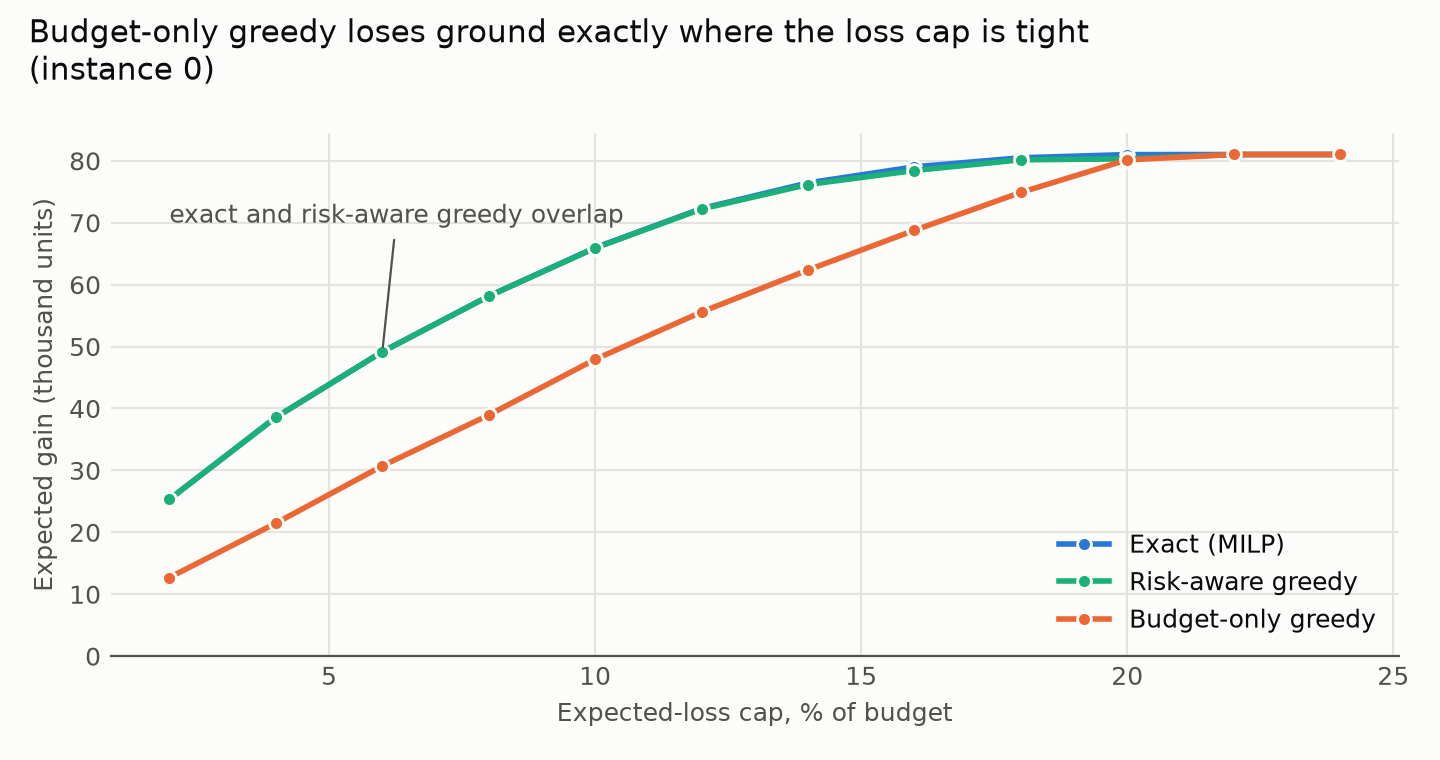
\includegraphics[width=0.78\textwidth]{fig_frontier.png}
\caption{Gain against the loss cap. The budget-only greedy rule falls behind when the cap is tight. A $\lambda$ fixed at the 15\% cap loses a few points at other caps.}
\label{fig:frontier}
\end{figure}

The budget-only rule reaches a median of \GreedyMed\% of the optimum, and only
\GreedyTightest\% when the loss cap is tight (Figure~\ref{fig:frontier}). The reason is that it
uses up the small loss allowance on high-risk farmers. When the loss cap is priced, the rule
reaches \GreedyRiskMed\% (worst case \GreedyRiskMin\%) with $\lambda$ searched and
\FixedMed\% (worst case \FixedMin\%) with the fixed $\lambda$. However, the fixed value does
not work equally well for other loss caps. Along the frontier it drops to
\FixedFrontierMin\% of the optimum. This is expected, because the price of a constraint
changes when the constraint becomes tighter or looser. In practice, a cheap allocation rule
works well only when it has a good estimate of $p_i$, and a repayment history could provide
this estimate.

\section{A revolving-fund simulation}

\paragraph{Model.} The simulation is individual-based. The farmers differ from each other and
are followed over several seasons, but they do not make decisions or act strategically. A fund
lends to 1{,}000 farmers in 20 villages for four seasons and lends out again what is repaid.
Farm sizes follow the forest-zone distribution in \citet{chamberlin2008} (median 1.62\,ha).
Yields and maize prices are the 2024 figures for Ghana (2.60\,t/ha and GH\textcent{}9{,}286/t;
\citealp{srid2024}), and 18\% of farmers do not respond to fertiliser \citep{ichami2019}. A
loan is diverted with a probability equal to the leakage rate of its custody model. Based on
Section~2, I assume 5\% for custodial wallets and 30\% when farmers hold their own keys.
Inputs increase the harvest by $r_i s_i\,(1-e^{-x/s_i})$, multiplied by a village weather
shock and an individual shock. The probability of default is
\begin{equation}
\Pr(\text{default}) = \sigma\!\left(\alpha + z_i + \delta\,\text{diverted} - \gamma\,\text{shock}
- \kappa\,(\text{gain}/\text{amount due} - 1)\right),
\end{equation}
where $z_i$ is a repayment type that the lender does not observe and the last term describes
repayment capacity.

\paragraph{The return to credit is the most uncertain input.} A simple agronomic calculation
(18\,kg of grain per kg of nitrogen at 2024 prices) gives a gross return of about 8.8 per
cedi. On-farm trials in northern Ghana gave about 3.6
\citep[Fosu and Dittoh 2011, as reported in][]{karlan2014}. A randomised controlled trial
(RCT) at farmer level found that cash grants increased harvest value by an amount that was not
statistically different from zero, and the authors conclude that uninsured risk is a bigger
constraint than credit \citep{karlan2014}. Because of this result I also use a low-return
scenario. The value 1.0 is my own conservative choice and not an estimate from the RCT. I run
all three values as separate scenarios. The baseline default rate is 25\%. It lies inside a
range whose upper end, 58\%, is the only figure from a Ghanaian pilot that I found
\citep{karlan2010}.

\paragraph{Policies.} I compare four policies: \emph{equal} amounts for everyone; the
risk-aware greedy rule with one pooled default rate (\emph{no history}); the same rule with a
logistic regression of default on the ledger history (\emph{ledger}); and the same rule when
each farmer's type is known (\emph{known type}). The last one is only a benchmark, because a
real lender cannot know the type. All policies use the same random draws, with \SimReps{}
replications per scenario.

\begin{table}[h]
\centering\small
\caption{Total harvest gain over four seasons (million GH\textcent{}, 2024 prices), ledger gain over no history (paired), and fund left after four seasons under the ledger policy.}
\label{tab:sim}
\setlength{\tabcolsep}{3.6pt}
\begin{tabular}{@{}llcccccc@{}}
\toprule
Return & Custody & Equal & No history & Ledger & Known type & Ledger vs none & Fund \\
\midrule
\SimRows
\bottomrule
\end{tabular}
\end{table}

\paragraph{Findings.} Pricing risk is better than equal amounts by \TargetLo--\TargetHi\% in
every scenario. The ledger history adds another \LedgerLo--\LedgerHi\%. The only exception is
the scenario with very high returns. There, defaults are rare and the history adds only
\LedgerMin\%, because there is not much to learn when almost everyone repays. Four seasons of
history give only part of the value of knowing the farmers. Under low returns, the history
adds \RctLedgerPct\%, while knowing the types would add \RctTypePct\%. Custody matters more
than the allocation rule. When farmers hold their own keys, the ledger policy loses
\CustodyLo--\CustodyHi\% of its gain. Finally, when returns are low, no policy keeps the
fund's capital. After four seasons the fund has \FundRctLo--\FundRctHi\% of its starting
capital under every policy, including the benchmark. This fits the result of
\citet{karlan2014} that risk, more than credit, limits these farmers. In that situation,
better targeting of credit is not enough.

\section{What the ledger history tells a lender}

To test the risk model on its own, I generate a panel of six seasons. In this panel the lender
gives equal amounts and the fund size stays constant, so there are always enough labelled
loans. Each season is predicted with a model that is trained only on the earlier seasons
(\RiskReps{} replications). I measure the ranking quality with the area under the ROC curve
(AUC).

\begin{table}[h]
\centering\small
\caption{Out-of-time AUC in season 6, trial-plot returns.}
\label{tab:auc}
\begin{tabular}{@{}lcc@{}}
\toprule
Features & Custodial & Self-custody \\
\midrule
\AucRows
\bottomrule
\end{tabular}
\end{table}

\begin{figure}[h]
\centering
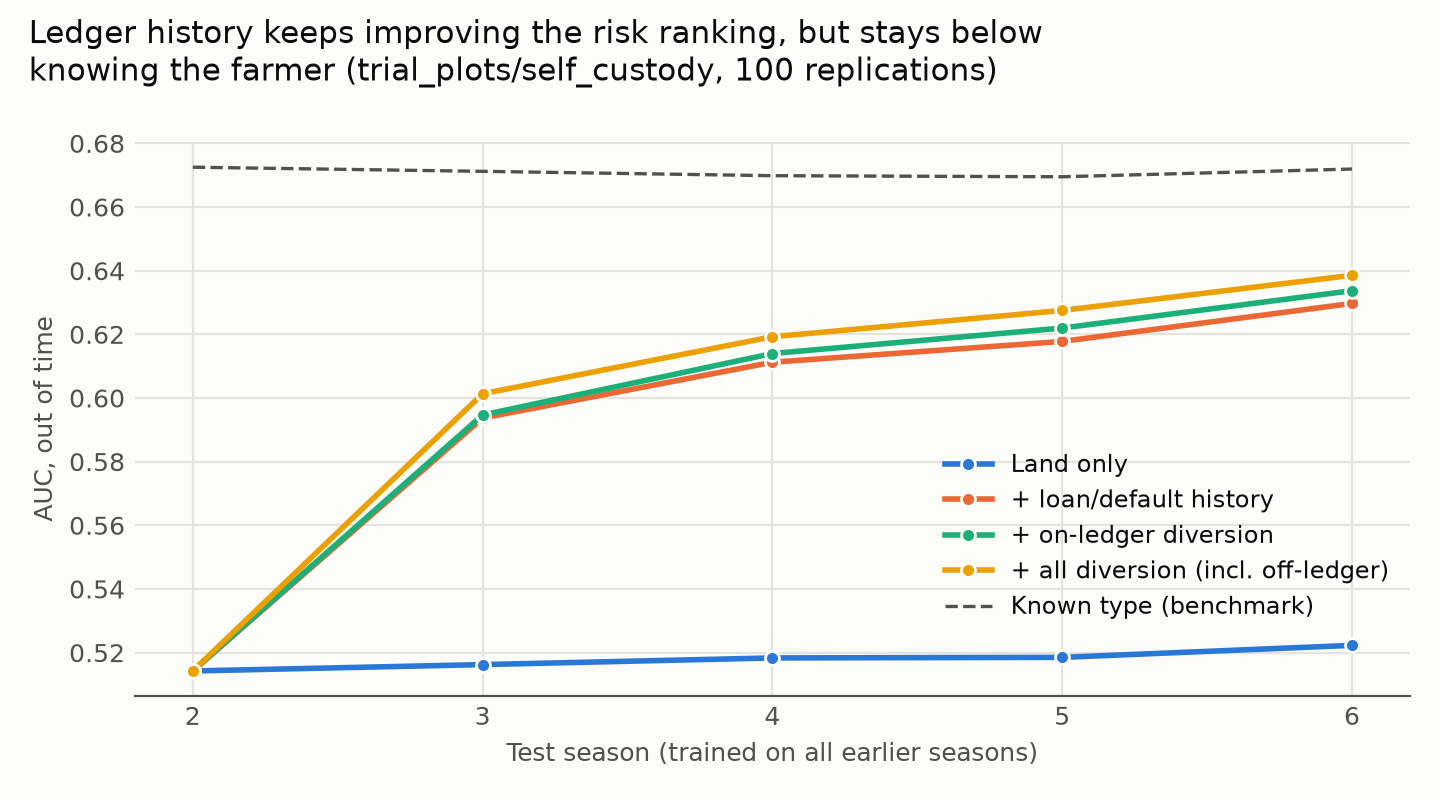
\includegraphics[width=0.78\textwidth]{fig_auc.png}
\caption{Out-of-time AUC by test season, self-custody.}
\label{fig:auc}
\end{figure}

Most of the information comes from the repayment record. With custodial wallets, five seasons
of loan and default history give the same AUC as the known-type benchmark
(Table~\ref{tab:auc}). Information about diversion adds almost nothing, even if the model
could see all diversion, which no ledger can do (S7). In the full simulation, changing the
on-ledger share of diversion from none to all changes the gain of the ledger policy only from
\ObsZero{} to \ObsFull{}. So it is more useful to prevent diversion through custody than to
try to detect it.

There are also some limitations. Gradient boosting performs worse than logistic regression on
this small dataset (\GbmAuc{} vs \LogAuc{}). The logistic model is over-confident at the
extremes. In the lowest decile it predicts \CalLoPred{} while the observed rate is
\CalLoObs{}, and in the highest decile it predicts \CalHiPred{} while the observed rate is
\CalHiObs{}. This matters because the allocation rule uses $p_i$ directly against the loss
cap. In addition, labels only exist for farmers who received a loan. A model trained on the
data of a selective lender therefore inherits that lender's choices. The usual solution is to
randomise part of the allocation.

\section{Robustness}

I moved each of the fifteen assumptions that have no source to a low and a high value
(\SensReps{} replications per point; Figure~\ref{fig:tornado}). No main result changes its
sign, except the survival of the fund. The remaining capital goes from \SensFundLo{} to
\SensFundHi{} times the starting capital, so I cannot make a claim about it in either
direction. The value of the ledger history is between +\SensLedgerLo\% and +\SensLedgerHi\%.
It almost disappears when defaults are rare (+\SensDefLow\%) or when the loss cap is loose
(+\SensCapLoose\%), and it is largest when defaults are high (+\SensDefHigh\%) or the cap is
tight (+\SensCapTight\%). In other words, the history is most useful when lending is most
difficult. Self-custody always costs \SensCustLo--\SensCustHi\% of the gain, and risk-aware
targeting is always better than equal amounts (+\SensTargetLo\% to +\SensTargetHi\%). The
on-ledger share of diversion has the smallest effect of all assumptions. Because I change one
assumption at a time, interactions between assumptions are not covered. A joint design would
be the next step.

\begin{figure}[h]
\centering
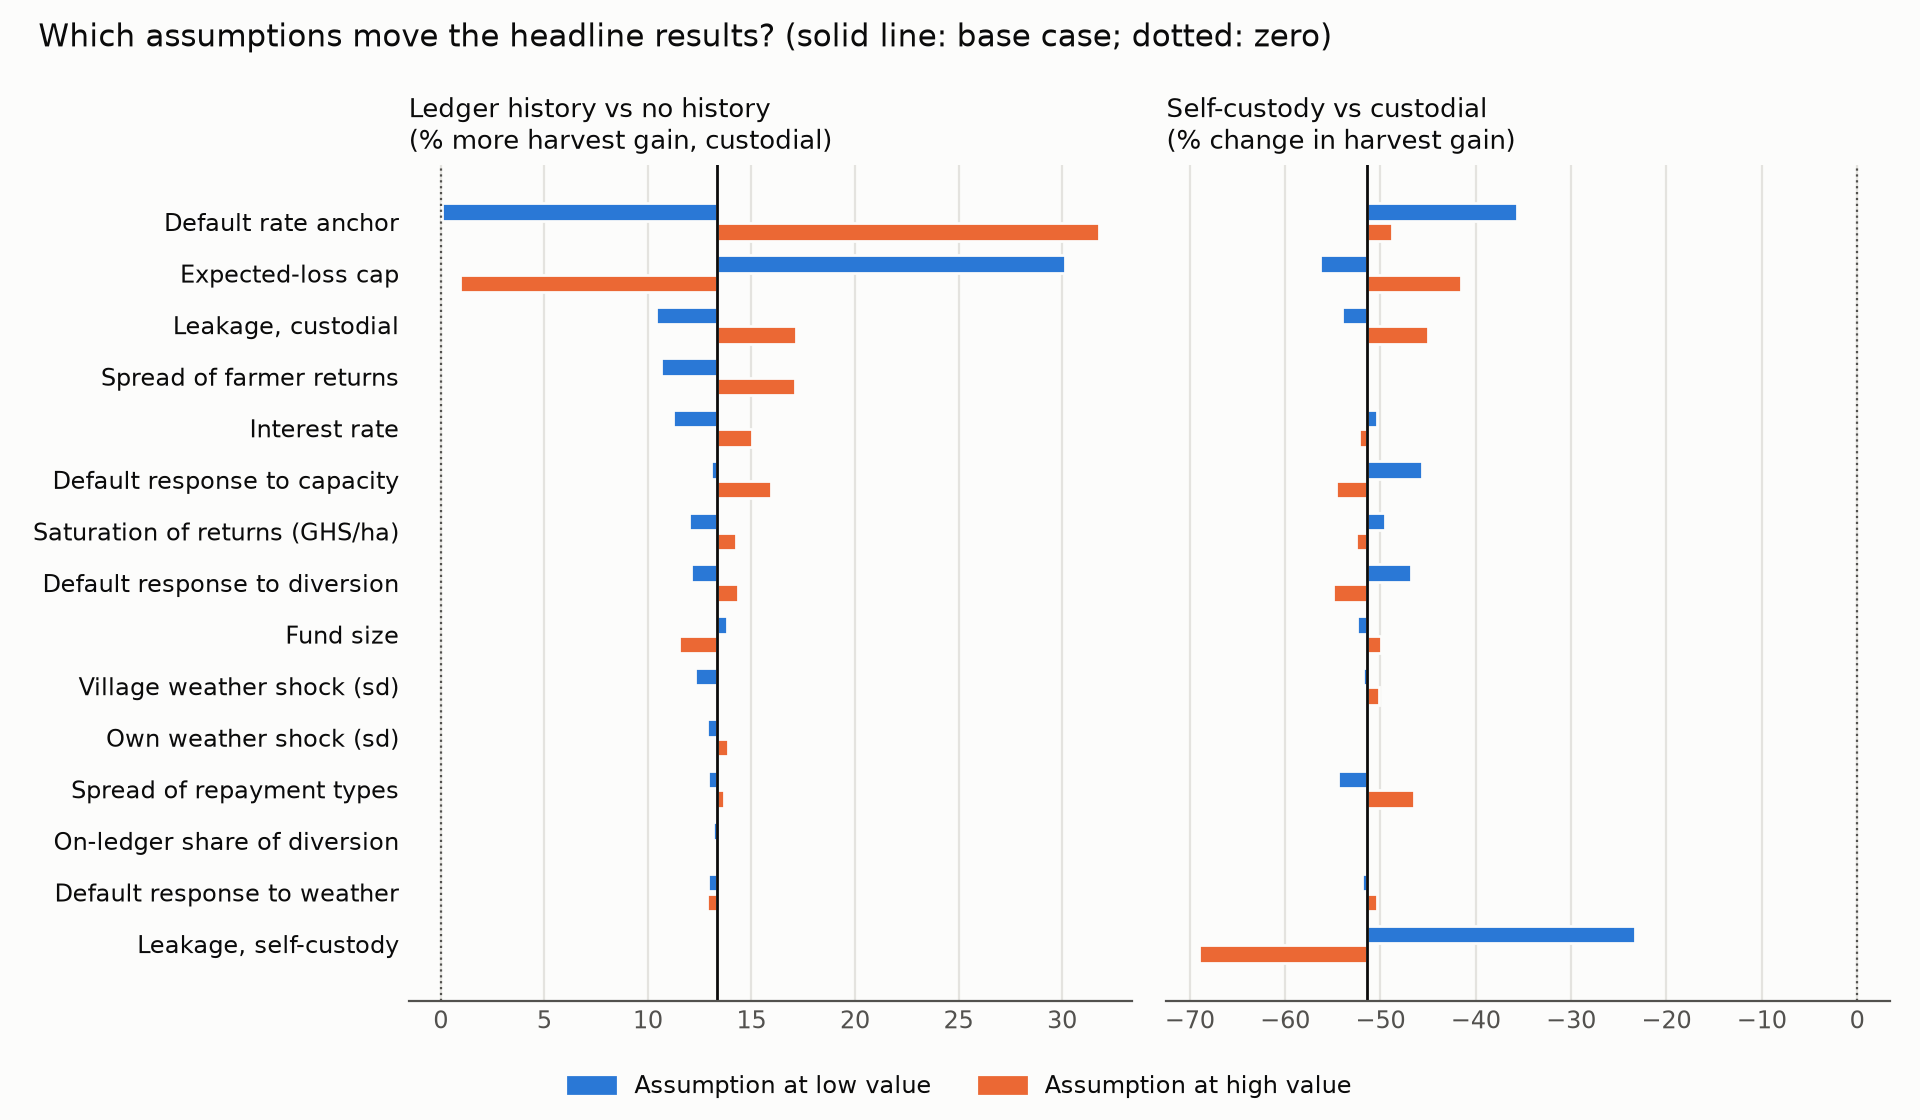
\includegraphics[width=0.92\textwidth]{fig_tornado.png}
\caption{One-at-a-time sensitivity of two headline results.}
\label{fig:tornado}
\end{figure}

\section{How a field experiment could test this}

The simulation gives hypotheses, not evidence. It points to two design choices, custody and
allocation, and both of them can be randomised. The design can follow the one that the Center
for Technology, Economics and Development (CTED) used to evaluate SMS price alerts in Ghana
\citep{neza2023,soldani2023}.

\begin{itemize}\itemsep0em
\item \textbf{Unit and spillovers.} Randomise village clusters instead of single farmers.
Farmers in one village share the same weather, and the escape routes from Section~2 are local,
because credit can move between neighbouring farmers (S4, S6) and through vendors (S7). In the
price-alert trial, villages with a lot of communication between them were merged before
randomisation (100 villages became 90 clusters) to stop information from moving from treatment
to control \citep{neza2023}. Here, trading links between villages could be used in the same
way.
\item \textbf{Balance.} Stratify before randomising, as that trial did by area and main crop
(eight strata). This prevents treatment from ending up mostly in the richer areas.
\item \textbf{Arms.} Custodial versus farmer-held wallets, cross-randomised with history-based
versus equal allocation. An additional arm with index insurance would test the result of
\citet{karlan2014} directly in a token-credit setting.
\item \textbf{Duration and spillovers to control.} Measure over several seasons. In the
price-alert trial, treated yam farmers received about 9\% higher prices in the first year,
crops with little bargaining showed no effect, and the authors point to longer-run spillovers
between villages \citep{soldani2023}. Credit also changes how vendors and traders behave, so
the effect after one season may not last.
\item \textbf{Outcomes and estimand.} Vendor payments (recorded on the ledger and almost free
to measure), yields from crop cuts, repayment and fund capital. The analysis would estimate
average treatment effects for each arm, with strata fixed effects and standard errors
clustered by village cluster. Since the simulation already predicts the expected signs, the
analysis should be pre-registered.
\end{itemize}

\begin{table}[h]
\centering\small
\caption{Illustrative minimum detectable effect on the default rate (percentage points), two arms, 50 borrowers per village, baseline default \PowerBaseDefault, $\alpha=0.05$, power 0.8, for three values of the intra-cluster correlation (ICC).}
\label{tab:power}
\begin{tabular}{@{}lccc@{}}
\toprule
Villages per arm & ICC 0.02 & ICC 0.05 & ICC 0.10 \\
\midrule
\PowerRows
\bottomrule
\end{tabular}
\end{table}

\noindent If we compare Table~\ref{tab:power} with the simulation, the custody effect on
default (\EffCustodyPP{} points) can be detected with about 40 villages per arm. The
allocation effect on default (\EffLedgerPP{} points) would need about \NeedLo{} to \NeedHi{}
villages per arm, for an intra-cluster correlation between 0.02 and 0.10. For this arm,
harvest gain or fund capital are more practical main outcomes. The intra-cluster correlations
here are assumptions, and data from a pilot would replace them.

\section{Limitations}

All farmer data are synthetic. The behavioural parameters, such as the size of the shocks,
how default reacts to type, diversion and capacity, and the leakage for each custody model,
are assumptions. I set ranges for them, but I did not estimate them. Harvest gain is the value
of output and not profit, because family labour and other input costs are not subtracted. The
landholding data are from 2005/06. The urea price behind the naive return scenario comes from
a source that I could not verify, so I use it only as an upper bound. I checked the testnet
behaviour with the amendments that were enabled on 2 October 2026, and this may change.
Nothing in this note describes how any deployed system works internally.

\section{Conclusion}

On the XRP Ledger, a spending restriction holds only if the farmer cannot sign transactions,
which in practice means a custodial wallet. A vendor who is willing to collude can still get
around any ledger rule. In the model, the main value of the ledger for a lender is a shared
repayment record that cannot be changed later. Seeing how the credit was spent adds much less.
The repayment record is most useful when lending is difficult, and it helps little when the
return to inputs is low. Only a field trial can show whether this is also true for real
farmers, and the simulation can help to choose a trial that would be informative.

\begin{thebibliography}{99}\small\itemsep0em
\bibitem[Chamberlin(2008)]{chamberlin2008} J.~Chamberlin. \emph{It's a Small World After All: Defining Smallholder Agriculture in Ghana}. IFPRI Discussion Paper 00823, 2008.
\bibitem[CTED(n.d.)]{cted} Center for Technology, Economics and Development, NYU Abu Dhabi. Blockchain Research. \url{https://www.nyucted.org/blockchain-research}, accessed 2 October 2026.
\bibitem[Ichami et al.(2019)]{ichami2019} S.~M.~Ichami, K.~D.~Shepherd, A.~M.~Sila, J.~J.~Stoorvogel, E.~Hoffland. Fertilizer response and nitrogen use efficiency in African smallholder maize farms. \emph{Nutrient Cycling in Agroecosystems} 113(1):1--19, 2019.
\bibitem[Karlan et al.(2010)]{karlan2010} D.~Karlan, E.~Kutsoati, M.~McMillan, C.~Udry. Crop price indemnified loans for farmers: a pilot experiment in rural Ghana. Working paper, November 2010.
\bibitem[Karlan et al.(2014)]{karlan2014} D.~Karlan, R.~Osei, I.~Osei-Akoto, C.~Udry. Agricultural decisions after relaxing credit and risk constraints. \emph{Quarterly Journal of Economics} 129(2):597--652, 2014.
\bibitem[MoFA-SRID(2025)]{srid2024} Ministry of Food and Agriculture, Statistics, Research and Information Directorate. \emph{Agriculture in Ghana: Facts and Figures 2024}.
\bibitem[Neza et al.(2023)]{neza2023} K.~Neza, Y.~Nyarko, A.~Orozco. Digital trading and market platforms: Ghana case study. In T.~Madon et al. (eds.), \emph{Introduction to Development Engineering}, ch.~9, pp.~221--245. Springer, 2023. doi:10.1007/978-3-030-86065-3\_9.
\bibitem[NYUAD(2026)]{nyuad2026} NYU Abu Dhabi. NYU Abu Dhabi receives generous grant for blockchain research. News release, August 2026. \url{https://nyuad.nyu.edu/en/news/latest-news/community-life/2026/august/blockchain-research-grant.html}, accessed 2 October 2026.
\bibitem[Soldani et al.(2023)]{soldani2023} E.~Soldani, N.~Hildebrandt, Y.~Nyarko, G.~Romagnoli. Price information, inter-village networks, and ``bargaining spillovers'': experimental evidence from Ghana. \emph{Journal of Development Economics} 164:103100, 2023.
\bibitem[Virtanen et al.(2020)]{scipy} P.~Virtanen et al. SciPy 1.0: fundamental algorithms for scientific computing in Python. \emph{Nature Methods} 17:261--272, 2020.
\bibitem[XRPL(a)]{xrpldepositauth} XRP Ledger documentation. Deposit Authorization. \url{https://xrpl.org/docs/concepts/accounts/depositauth}, accessed 2 October 2026.
\bibitem[XRPL(b)]{xrpldomains} XRP Ledger documentation. Permissioned Domains. \url{https://xrpl.org/docs/concepts/tokens/decentralized-exchange/permissioned-domains}, accessed 2 October 2026.
\end{thebibliography}

\end{document}
